\section{Exploratory Data Analysis}\label{sec:eda}
We begin by giving an overview of the data recorded in the study. A description of each variable is shown in \cref{tab:var.decription}. Note that a higher GSI score indicates a higher level of mental distress. There are five recordings of the GSI score (response) for each participant, measured respectively at the beginning of the study (0), and three (3), six (6), eighteen (18), and sixty (60) months later, as indicated by the month variable. While none of the other variables change over time, the repeated GSI measurements make this study longitudinal.\\\\
Of all 271 participants in the study, 57.6\% were randomly placed in the intervention group and the remaining 42.4\% were in the control group. Excluding those whose gender are unknown, 34.1\% of the participants are male and 65.9\% are female (\cref{tab:summ.stat.cat}). While the split between the two treatment groups is roughly balanced, there may be a slight underrepresentation of male participants in the data. However, since there are as many as 271 participants in total, there are still many participants that are male. Therefore there should not be a major impact of the unbalanced gender proportions.
\begin{table}[H]
\centering
\begin{tabular}{|l|l|}
\hline
SN & subject number \\
\hline
treatment & treatment received by each subject ($1$ for intervention and $2$ for control)\\
\hline
month & measurement time (in month)\\
\hline
gender & gender of each subject ($1$ for male and $2$ for female)\\
\hline
education & education received by each subject (in years)\\
\hline
GSI & Global Severity Index: an index indicating level of mental distress\\
\hline
\end{tabular}
\caption{Description of all variables recorded in the study}
\label{tab:var.decription}
\end{table}
\noindent The means and standard deviations of all continuous variables are shown in \cref{tab:summ.stat.cont}. We see that the GSI scores decreases over time while the corresponding standard deviations roughly stay consistent. Another observation is that the GSI scores are much smaller in magnitude compared to the education and month variables. This difference in scale may make the estimated effects of these explanatory variables on GSI unusually small. To aviod getting results of low interpretability, the GSI scores are scaled by a factor of ten (10) for the remainder of this report.\\\\
A common issue in longitudinal studies is missing data. As expected, with the GSI scores recorded over the span of five years, some of the response values are missing. This is common as some of the participants may have dropped out of the study for various reasons. In addition, some participants' gender and amount of education received are also missing. The count of missing values and the corresponding proportion of missing values are shown in \cref{tab:missing.rate}. It is clear that more participants dropped out of the study as time went on. With the missing rates as high as 38.7\%, it is important that we address the sensitivity of our subsequent analysis to these missing data in \cref{sec:confirmatory}.
\begin{table}[h]
\begin{minipage}{0.5\textwidth}
\centering
\resizebox{\linewidth}{!}{
\begin{tabular}{|l|l|l|l|l|l|l|}
\hline
& education & GSI (0) & GSI (3) & GSI (6) & GSI (18) & GSI (60)\\
\hline
mean & 13.705 & 1.125 & 1.036 & 0.854 & 0.834 & 0.780 \\
\hline
sd & 2.360 & 0.722 & 0.702 & 0.638 & 0.559 & 0.625 \\
\hline
\end{tabular}
}
\caption{Summary statistics for continuous variables}
\label{tab:summ.stat.cont}
\end{minipage}
\hfill
\begin{minipage}{0.5\textwidth}
\centering
\resizebox{\linewidth}{!}{
\begin{tabular}{|l|l|l|l|l|l|l|l|}
\hline
& gender & education & GSI (0) & GSI (3) & GSI (6) & GSI (18) & GSI (60)\\
\hline
count & 4 & 7 & 10 & 38 & 52 & 105 & 98 \\
\hline
proportion & 0.015 & 0.026 & 0.037 & 0.140 & 0.192 & 0.387 & 0.362 \\
\hline
\end{tabular}
}
\caption{Missing rates of all variables in the study}
\label{tab:missing.rate}
\end{minipage}
\end{table}
\subsection{Visualization of GSI}
We now use side-by-side boxplots to get a rough idea of how the two main questions laid out in \cref{sec:introduction} can be answered. We first visualize the changes in the GSI scores over time for both the intervention group and the control group. Note that the p-values of the ANOVA and Kruskal-Wallis tests are also included in the caption for each of the two groups. In this case, ANOVA, as a generalization of the commonly known t-test, tests whether the mean GSI scores are the same across each of the five time points. Since ANOVA assumes the data to be normally distributed, which may not hold, the Kruskal-Wallis test is also conducted as a non-parametric alternative. The Kruskal-Wallis test does not make the normality assumption and is relatively robust against outliers, which can be seen to be present in \cref{fig:boxplot.over.time}. The Kruskal-Wallis test here serves as a reference to check the reliability of the results from the ANOVA tests.\\\\
From \cref{fig:boxplot.over.time}, we see that a downward trend of GSI over time is present in both groups. At the same time, the p-values from the ANOVA and Kruskal-Wallis tests (all $<0.021$) indicate that there is moderate to strong evidence against that the mean GSI scores are the same across all five time points. It is then suggested that the participants' mental distresses in both groups decrease significantly over time.
\begin{figure}[H]
\centering
\begin{subfigure}{.4\textwidth}
  \centering
  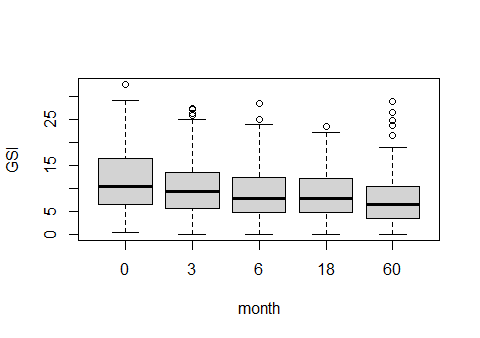
\includegraphics[width=1\linewidth]{../../plots/box_over_time_treatment.png}
  \caption{intervention group (ANOVA: 0, Kruskal-Wallis: 0)}
\end{subfigure}
\begin{subfigure}{.4\textwidth}
  \centering
  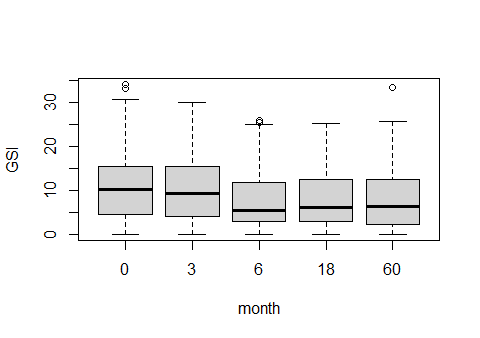
\includegraphics[width=1\linewidth]{../../plots/box_over_time_control.png}
  \caption{control group (ANOVA: 0.021, Kruskal-Wallis: 0.006)}
\end{subfigure}
\caption{Side-by-side boxplots of the GSI scores across measurement times for each treatment group}
\label{fig:boxplot.over.time}
\end{figure}
\noindent To visualize whether the GSI scores are different between the intervention group and the control group at each of the five time points, we again use side-by-side boxplots. This is shown in \cref{fig:boxplot.between.groups}. Similarly, the p-values of two-sample t-tests and Wilcoxon tests are included in the caption to quantify the evidence we have against that the mean GSI scores are equal. Again, since the t-test assumes the data to be normally distributed and may be sensitive to outliers, the Wilcoxon test serves as a robust alternative. By the boxplots in \cref{fig:boxplot.between.groups}, the GSI scores of the two groups do not seem to differ much in any of the five times points. The p-values from the t-tests and Wilcoxon tests also indicate that, for the most part, there is no evidence against that the mean GSI scores between the two groups are the same.
\begin{figure}[H]
\begin{subfigure}{.19\textwidth}
  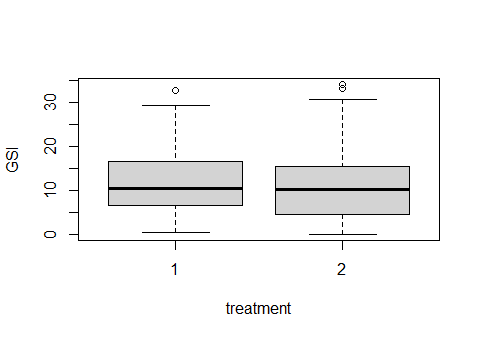
\includegraphics[width=1\linewidth]{../../plots/box_between_group_0.png}
  \caption{baseline (t-test: 0.457, Wilcoxon: 0.271)}
\end{subfigure}
\begin{subfigure}{.19\textwidth}
  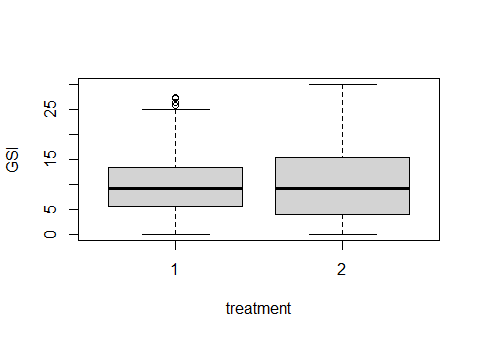
\includegraphics[width=1\linewidth]{../../plots/box_between_group_3.png}
  \caption{3 months (t-test: 0.995, Wilcoxon: 0.489)}
\end{subfigure}
\begin{subfigure}{.19\textwidth}
  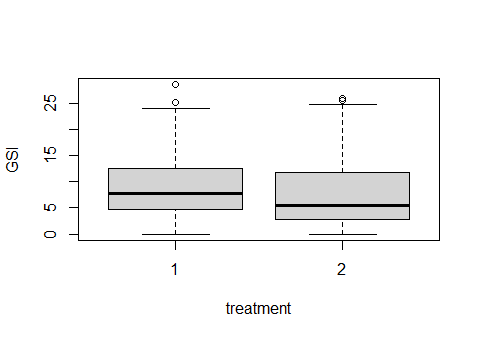
\includegraphics[width=1\linewidth]{../../plots/box_between_group_6.png}
  \caption{6 months (t-test: 0.332, Wilcoxon: 0.084)}
\end{subfigure}
\begin{subfigure}{.19\textwidth}
  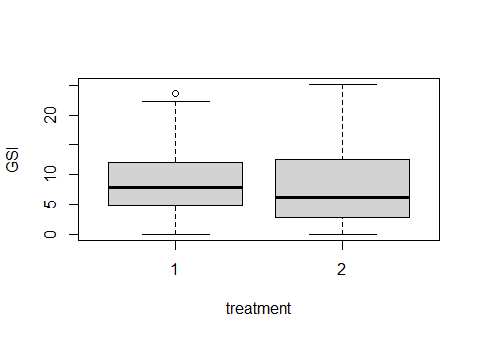
\includegraphics[width=1\linewidth]{../../plots/box_between_group_18.png}
  \caption{18 months (t-test: 0.405, Wilcoxon: 0.167)}
\end{subfigure}
\begin{subfigure}{.19\textwidth}
  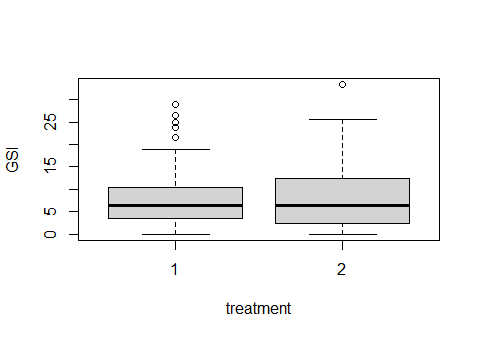
\includegraphics[width=1\linewidth]{../../plots/box_between_group_60.png}
  \caption{60 months (t-test: 0.826, Wilcoxon: 0.831)}
\end{subfigure}
\caption{Side-by-side boxplots of the GSI scores between two treatment groups across measurement times}
\label{fig:boxplot.between.groups}
\end{figure}
\subsection{Association between Explanatory Variables}
\begin{wrapfigure}{r}{.4\textwidth}
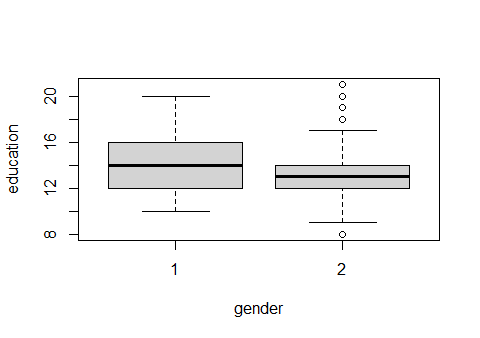
\includegraphics[width=1\linewidth]{../../plots/box_correlation.png}
\caption{Side-by-side boxplot of education between the two genders (t-test: 0.014, Wilcoxon: 0.045)}
\label{tab:boxplot.correlation}
\end{wrapfigure}
Before summarizing our preliminary conclusions, it is worth inspecting the association between the two explanatory variables: gender and education. Since the gender variable is categorical, instead of computing the Pearson correlation coefficient, we use a side-by-side boxplot to study the association between the two variables \cref{tab:boxplot.correlation}. Again, the p-values of t-test and Wilcoxon test are included in the caption. The plot suggests that the male participants as a group has received more education in terms of the number of years. The p-values (0.014 and 0.045) also indicates that there is moderate to strong evidence that the mean amount of education received in years among the male participants is different than that of the female participants. It is then possible that one of the two explanatory variables is enough to explain much of the variability present in the GSI scores of the corresponding participants. It is then worth inspecting whether including both of these explanatory variables leads to better fit models in \cref{sec:confirmatory}.

\subsection{Preliminary Conclusions}
From the above graphical displays of the response variable, it is suggested that the participants' mental distresses in both the intervention group and the control group decrease over time. However, there does not seem to be a clear indication that the mental health intervention leads to a lower level of mental distress when compared to the control group. It is worth noting that the above preliminary conclusions are drawn without considering the gender and amount of education received of each participant. It is possible that these two explanatory variables exaggerate the effect of time or mask the effect of the mental health intervention on mental distress. Therefore, further analysis using various statistical models needs to be conducted to check the reliability of the conclusions drawn from the above exploratory data analysis.